\documentclass{beamer}
\usepackage{beamerthemesplit} % new 
\usepackage{amsmath}
\begin{document}
\title{Text-to-SQL Semantic Parsing} 
\author{Group 4 \\ Nguyen Tan Viet \\ Ngo Quoc Bao}

\date{\today} 
\frame{\titlepage} 


\frame{\frametitle{Problem} 
\begin{block}{Definition of problem}
\vspace{0.5em}
Given a natural language $Q$ and the schema $S = \langle \mathcal{T},\mathcal{C}\rangle$ for a relational database, the parser needs to generate the corresponding SQL query $Y$. The schema consists of tables $\mathcal{T} = \{t_1,..,t_N\}$ and fields $\mathcal{C} =\{c_{11},...,c_{1|T_1|},...,c_{n1},...,c_{N|T_N|} \}$.Each table $t_i$ and each field $c_{ij}$ has a textual name. Some fields are primary keys, used for uniquely indexing each data record, and some are foreign keys, used to reference a primary key in a different table. In addition, each field has a data type, $\tau\in\{number,text,time,boolean,etc\}$
\vspace{0.5em}
\end{block}
}

\frame{\frametitle{Problem} 
\begin{block}{Definition of problem: SQL Cross domain database}
\begin{figure}
   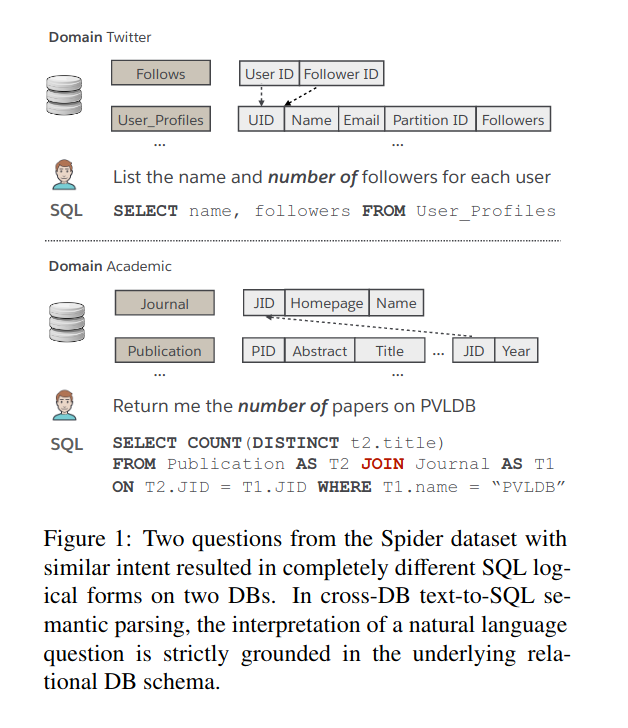
\includegraphics[width=\linewidth,height=7cm]{./image/2.png}
\end{figure}
\end{block}
}


\frame{\frametitle{Literal review}
\begin{block}{Represent schema as Graph}
\begin{figure}
   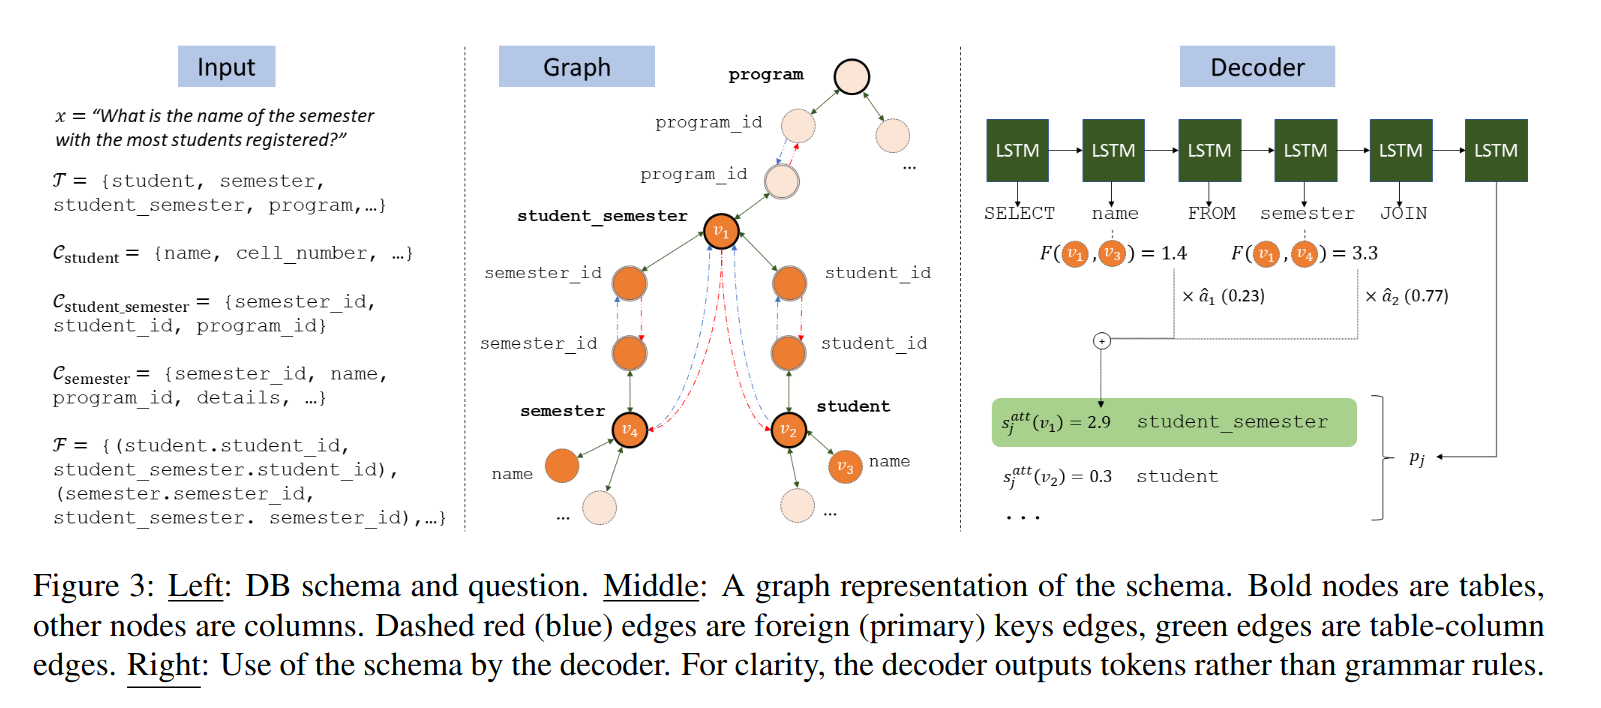
\includegraphics[width=\linewidth,height=6.5cm]{./image/3.png}
\end{figure}
\end{block}}


\frame{\frametitle{Literal review}
\begin{block}{Represent schema as Graph}
\vspace{0.5em}
\begin{enumerate}
\item Use decoder uses graph structue to guide decoding
\item E.g: LSTM generates token by token when decoder generates token schema $\nu$, the subsequent generated tokens can be considered as $\tau(\nu)$.
\item For example to generate SQL query SELECT FROM $student$ WHERE $student.lastname == "Nguyen"$. Decoder first generates SELECT FROM then the next token must be table name according to grammar rules.
\end{enumerate}
\vspace{0.5em}
\end{block}}

\frame{\frametitle{Literal review}
\begin{block}{Represent problem as Seq2seq models for text2SQL}
\vspace{0.5em}
\begin{enumerate}
\item Encoder encodes natural question,sequential schema and translates to SQL logical form.
\item Shaw et al.(2020) showed T5 model with 3 billion parameters achieves state of the art on spider. 
\end{enumerate}
\vspace{0.5em}
\end{block}}

\frame{\frametitle{Literal review}
\begin{block}{Use DB content}
\vspace{0.5em}
\begin{figure}
   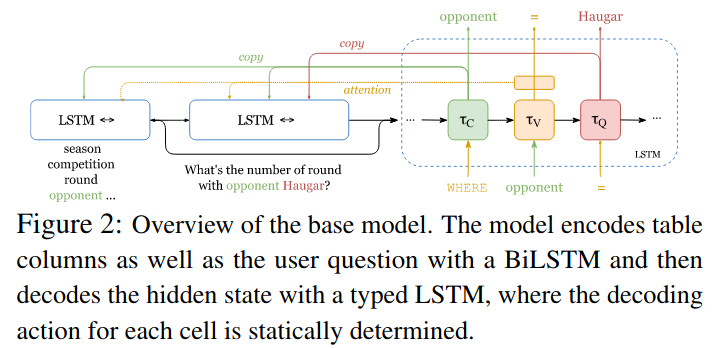
\includegraphics[width=\linewidth,height=6.5cm]{./image/4.png}
\end{figure}
\vspace{0.5em}
\end{block}}


\frame{\frametitle{Literal review}
\begin{block}{Use DB content- RAT SQL}
\vspace{0.5em}
\begin{figure}
   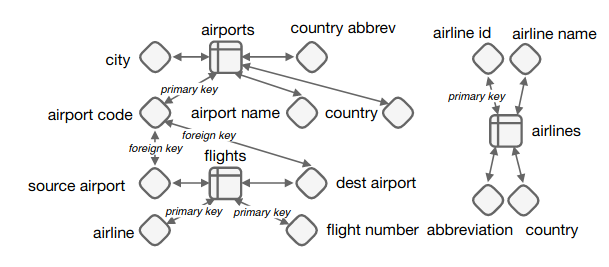
\includegraphics[width=\linewidth,height=6.5cm]{./image/5.png}
\end{figure}
\vspace{0.5em}
\end{block}}

\frame{\frametitle{Literal review}
\begin{block}{Use DB content- RAT SQL}
\vspace{0.5em}
\begin{figure}
   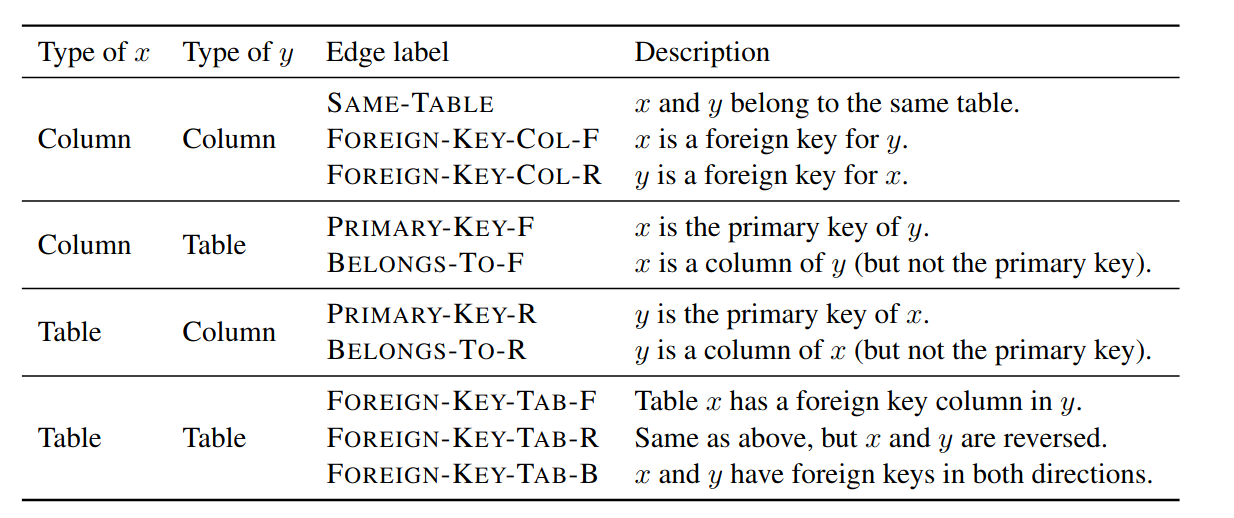
\includegraphics[width=\linewidth,height=6cm]{./image/6.png}
\end{figure}
\vspace{0.5em}
\end{block}}

\frame{\frametitle{Literal review}
\begin{block}{Use DB content- RAT SQL}
\begin{enumerate}
\item RAT-SQL uses relational transformers to encode relations of tokens. \\ $e^{(h)}_{ij}=\frac{x_{i}W_{Q}^{(h)}(x_{j}W_{K}^{h}+r_{ij}^{K})^{T}}{\sqrt{d_{z}/H}}$ \\
$z_{i}^{(h)}=\sum_{j=1}^n\alpha_{ij}^{(h)}(x_{j}W_{V}^{(h)}+r^{V}_{ij})$
\item RAT-SQL performs schema-linking, name-based linking, value-based linking based on relation types above. 
\item Encode schema and question is independent.
\end{enumerate}
\end{block}}


\begin{frame}[t]{New point in research}\vspace{10pt}
\begin{enumerate}
\item  Model has acess to value of each field called picklists (e.g $Property\_type\_code$ can have one of the following values $\{"Apartment","Field","House","Shop","Other"\}$ ) \\
$\rightarrow$ protect individual data record and sensitive fields such as User IDs or credit numbers.
\item Use LSTM-based pointer generator with multihead-attention as decoder
\end{enumerate}
\end{frame} 
\begin{frame}[t]{New point in research}\vspace{10pt}
\begin{block}{Question-schema serialization and encoding}
\vspace{0.5em}
\begin{enumerate}
\item $X = [CLS],Q,[SEP],[T],t_{1},[C],c_{11},...,c_{1|T_1|},$\\$[T],t_{2},[C],c_{21},...,c_{N|T_N|},[SEP]$ \\
\item X is encoded with Bert
\item Folowed by a directional LSTM $\textbf{h}_{X}\in\mathbb{R}^{|X|xn}$ 
\item The question $\textbf{h}_{X}$ is passed through another bi-LSTM $\textbf{h}_{Q}\in\mathbb{R}^{|Q|xn}$ 
\item Dense lookup features to represent meta-data of schema $f_{pri}\in\mathbb{R}^{2xn}$, $f_{for}\in\mathbb{R}^{2xn}$, $f_{type}\in\mathbb{R}^{|\tau|xn}$
\vspace{0.5em}
\end{enumerate}
\end{block}
\end{frame}

\begin{frame}[t]{New point in research}\vspace{10pt}
\begin{block}{Question-schema serialization and encoding}
\vspace{0.5em}
Meta-data features and base encoding are fused via a feed-forward layer $g(\mathbb{R}^{4n}\rightarrow\mathbb{R}^{n})$:
\begin{enumerate}
\item $\textbf{h}^{t_{i}}_{S} = g([\textbf{h}^{p}_{X};\textbf{0};\textbf{0};\textbf{0}])$
\item $\textbf{h}^{c_{ij}}_{S} = g([\textbf{h}^{q}_{X};f^{u}_{pri},f^{v}_{for},f^{w}_{type}])$ \\ $=ReLU(\textbf{W}_{g}[\textbf{h}^{q}_{X};f^{u}_{pri},f^{v}_{for},f^{w}_{type}]+\textbf{b}_{g})$
\item $\textbf{h}_{S} = [\textbf{h}^{t_{1}},...,\textbf{h}^{t_{|\tau|}},\textbf{h}^{c_{11}},...,\textbf{h}^{c_{N|T_{N}|}}] \in \mathbb{R}^{|S|xn}$
\vspace{0.5em}
\end{enumerate}
\end{block}
\end{frame}

\begin{frame}[t]{New point in research}\vspace{10pt}
\begin{block}{Bridging}
\vspace{0.5em}
Anchor text, perform fuzzy matching between question $Q$ and the picklists of each field, if found the matched values in DB, the mathched field values are inserted in X, succeeding corresponding field name and seperated by token $[V]$.
\begin{figure}
   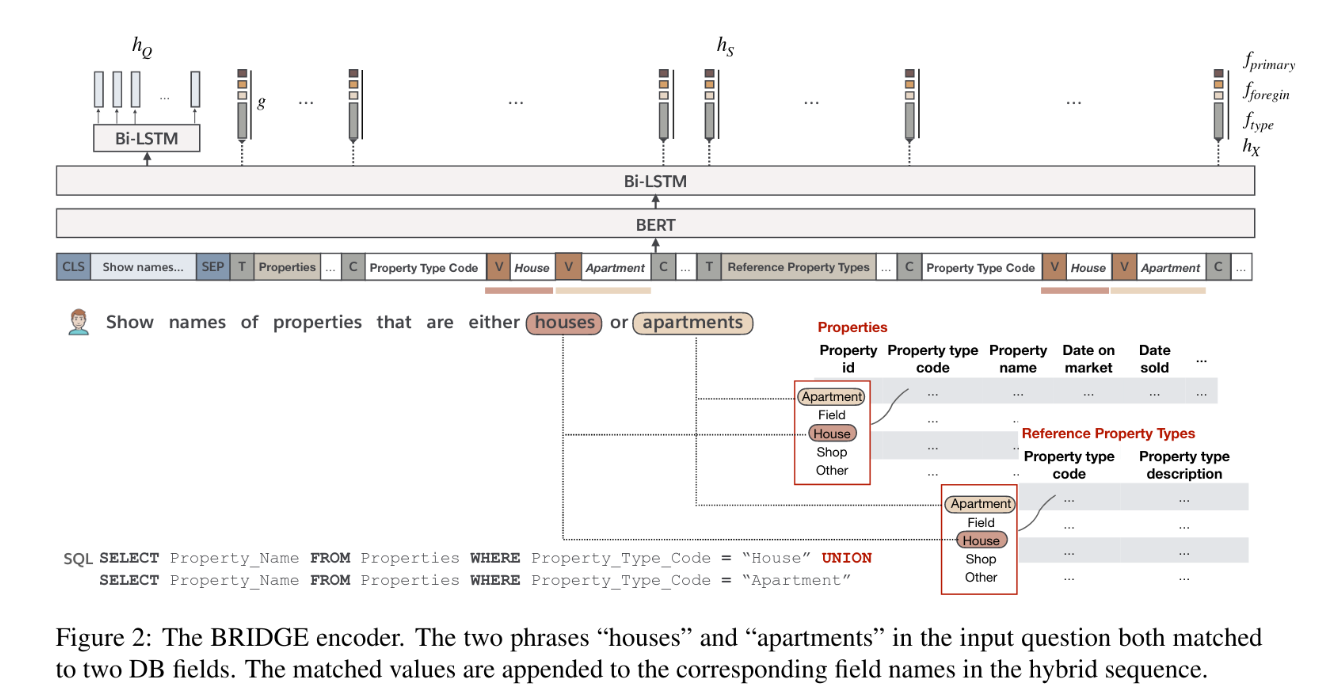
\includegraphics[width= 0.7\linewidth]{./image/1.png}
\end{figure}
\vspace{0.5em}
\end{block}
\end{frame}

\begin{frame}[t]{New point in research}\vspace{10pt}
\begin{block}{Decoder}
\vspace{0.5em}
The decoder starts
from the final state of the question encoder. At
each step, the decoder performs one of the follow-
ing actions: generating a token from the vocabulary
$V$, copying a token from the question $Q$ or copying
a schema component from $S$.\\
Mathematically, at each step $t$, given the decoder
state $s_{t}$ and the encoder representation $[h_{Q}; h_{S} ]\in
\mathbb{R}^{(|Q|+|S|)xn}$\\\vspace{5pt}
$e_{tj}^{(h)} = \frac{s_{t}W^{(h)}_{U}(h_{j}W^{(h)}_{V})^\top}{\sqrt{n/H}};\space \alpha_{tj}^{(h)}=\underset{j}{softmax}\{e_{tj}^{(h)}\}$\\ \vspace{5pt}
$z_{t}^{(h)} = \sum^{|Q|+|S|}_{j=1}\alpha_{tj}^{(h)}(h_{j}W^{(h)}_{V});z_{t}=[z_{t}^{(1)},...,z_{t}^{(H)}]$\\\vspace{5pt}
$p^{t}_{gen}=sigmoid(s_{t}W^{s}_{gen}+z_{t}W^{z}_{gen}+b_{gen})$\\\vspace{5pt}
$p^{t}_{out} = p^{t}_{gen}P_{\mathcal{V}}(y_{t})+(1-p^{t}_{gen})\sum_{j: \overset{\sim}{X}_{j}=y_{t}}\alpha_{tj}^{(H)})$
\vspace{0.5em}
\end{block}
\end{frame}

\begin{frame}[t]{New point in research}\vspace{10pt}
\begin{block}{Schema-Consistency Guided Decoding}
\vspace{0.5em}
a simple pruning strategy for sequence
decoders, based on the fact that the DB fields ap-
peared in each SQL clause must only come from
the tables in the FROM clause. \\
\textbf{Lemma 1} Let $Y_{exec}$ be a SQL query with clauses
arranged in execution order, then any table field in
$Y_{exec}$ must appear after the table.\\
As a result, we adopt a binary attention mask $\xi$\\
$\overset{\sim}{\alpha}_{t}^{(H)}=\alpha_{t}^{(H)} . \xi$\\
which initially has entries corresponding to all
fields set to 0 Once a table $t_{i}$ is decoded, 
all entries in $\xi$ corresponding to that table to 1, allows the decoder to only search in the space
specified by the condition in Lemma 1 with little
overhead in decoding speed.
\vspace{0.5em}
\end{block}
\end{frame}



\frame{\frametitle{experiment result}}

\frame{\frametitle{ablation study}}

\frame{\frametitle{error analysis}}


\frame{\frametitle{Demo}}

\end{document}